\documentclass[conference]{IEEEtran}
% \IEEEoverridecommandlockouts
% The preceding line is only needed to identify funding in the first footnote. If that is unneeded, please comment it out.
\usepackage{cite}
\usepackage{amsmath,amssymb,amsfonts}


\usepackage{hyperref}
%\usepackage[ngerman]{cleveref}
\usepackage[english]{cleveref}

% \usepackage{algorithmic}
\usepackage{graphicx}
\usepackage{textcomp}
\usepackage{xcolor}
\def\BibTeX{{\rm B\kern-.05em{\sc i\kern-.025em b}\kern-.08em
    T\kern-.1667em\lower.7ex\hbox{E}\kern-.125emX}}
\begin{document}

\title{Text Analytica: cloud-based document analysis\\}

\author{\IEEEauthorblockN{Florian Bauer}
\IEEEauthorblockA{\textit{Department of Computer Science} \\
\textit{University of Bristol}\\
Bristol, United Kingdom \\
ya18048@bristol.ac.uk}
\and
\IEEEauthorblockN{Nathalie Pett}
\IEEEauthorblockA{\textit{Department of Computer Science} \\
\textit{University of Bristol}\\
Bristol, United Kingdom \\
aq18034@bristol.ac.uk}
}

\maketitle

\begin{abstract}
Text Analytica is a cloud-based web service for document analysis. The prototype introduced and discussed in this report currently accepts txt file uploads and extracts the three most common words. The web service is hosted on \textit{Microsoft Azure} and makes use of serveral cloud computing technologies. The functionality of Text Analytica is containerised into Docker containers orchestrated by a Kubernetes cluster. The data generated from the text analysis is stored in an \textit{Azure Cosmos DB}. All technologies used were chosen for their positive impact on scalabitity. The scalability of Text Analytica was examined by the means of a load test. The source code is available at https://github.com/darkcookie298/CloudComputing. The application can be run online at http://textanalytica.lukaspman.io/.
\end{abstract}

\section{Introduction}
\label{sec:intro}
Text Analytica is a cloud-based web service aiming to support the analysis of text documents. For the purpose of this coursework a prototype has been developed, deployed and evaluated using different cloud computing technologies. In the remainder of this section, the concept of Text Analytica is discussed as well as the limitations of the implemented prototype. \Cref{sec:platform-choice} explores the reasons for choosing Microsoft's cloud services over Oracle's. Afterwards in \Cref{sec:system-architecture} the system architecture and technologies used for the project are explained in more detail. Different aspects of the service's scalability are addressed in \Cref{sec:scalability}, including evidence of the performance of the service under load. Lastly future improvements of Text Analytica are proposed in \Cref{sec:future-improvements}.

\begin{figure*}[ht!]
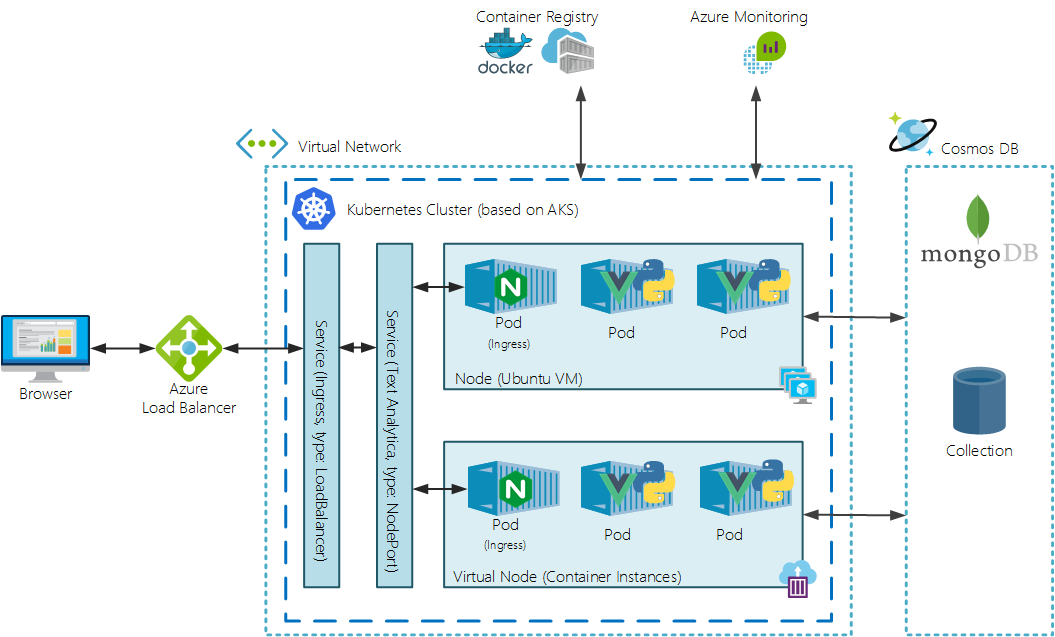
\includegraphics[width=150mm]{img/architectur.png}
\caption{Text Analytica's system architecture: The main components of the system are a Kubernetes cluster based on AKS, orchestrating the containers running Text Analytica and a \textit{Microsoft Cosmos DB}, storing the results of the analysis. Each container is encapsulated by its own Kubernetes Pod. The images to build new containers can be pulled from the \textit{Docker Hub} container registry. Azure monitoring is used to monitor the health of the cluster and its components. The Kubernetes cluster is exposed for external access through an \textit{Azure Load Balancer}.}
\label{img:architecture}
\end{figure*}

\subsection{Vision}
University students are often faced with an abundance of resources regarding specific units or even certain topics within a unit. These range from lecture notes or slides to personal notes and additional scientific papers as well as e-books or extracts thereof. The first step in the exploration process is for students to familiarise themselves with these materials by identifying the documents' key aspects and discovering links between different sources. This is what Text Analytica ultimately aims to facilitate.

More specifically the functionalities of Text Analytica could include tagging, keyword search, suggestions of related documents based on textual analysis and eventually the generation of short summaries, all based on user-supplied PDF documents. These functionalities render Text Analytica a useful tool for many scenarios in which people are confronted with a large number of different and possibly complex text sources, e.g. in the context of management decisions in industry or business / commerce.

\subsection{Limitations of the submitted prototype}
\label{subsec:limits}
The focus of this coursework assignment was to deploy an application using different cloud services and explore its scalability, while remaining within the proposed time frame. Therefore, the functionality of the submitted prototype was stripped down to a minimum.

To skip the step of extracting machine-readable text from PDFs by applying OCR techniques, currently users are only able to upload simple txt documents. These files are parsed and analysed. At this point the analysis merely tags the system entries with the three most common words in the text. The content of the text file is stored as a string as part of the analysis, therefore currently there is no reason to store the actual files within the application and they are discarded after being processed. Additionally, no user account and login functionality has not yet been implemented.

\section{Platform choice}
\label{sec:platform-choice}
The considerations detailed below eventually led to choosing \textit{Microsoft Azure} instead of the services introduced in the lectures by Oracle to remain within the proposed time scope for the coursework.

\subsection{Setup}
\label{subsec:setup}
Given the tutorials in class as well as the $\pounds 3,500$ in credits granted to us for \textit{Oracle Cloud}, we initially intended to build our application based on their services. We started trying to set up a Kubernetes cluster with the \textit{Terraform} command line tool, as was recommended to us. However, after having spent a significant amount of time on installing all necessary tools, e.g. \textit{Terraform} itself, the \textit{Terraform Provider OCI}\cite{TerraformProviderOCI} and the \textit{Terraform Kubernetes Installer for Oracle Cloud} \cite{TerrafromK8sInstaller}, we failed to set up an easy example cluster due to reaching service limits. These limits restrict how many instances of a specific resource in a zone one can use. To increase the limit a ticket with Oracle support must be opened, a process which is very slow and inconvenient. While \textit{Microsoft Azure} does also have such limits \cite{AzureLimits}, they are far more generous and therefore allowed us to work more efficiently, without depending on the reply of third parties.

Another inconvenience of \textit{Oracle Cloud} is the unstructured and inconsistent user interface of the control panel. This became especially apparent when comparing it to the user interfaces of Amazon, as demonstrated in the lecture, and Microsoft, which was eventually used to configure the cluster and database for Text Analytica. In addition to this, Azure made it very easy to work with third party SDKs as it provides good integration of these services within their own ecosystem.

\subsection{Documentation and support}
\label{subsec:docandsupport}
Working with one of \textit{"the big three"} providers of cloud computing, that is \textit{Google Cloud}, \textit{Amazon Web Services} or \textit{Microsoft Azure} comes with considerable advantages, when it comes to documentation and support. Not only are there large numbers of tutorials, answered questions on \textit{Stackoverflow} and blog articles on their technologies, but they also come with very comprehensive documentations. The number of tutorials using Oracle's cloud services, however, was relatively small, making it difficult for beginners to get started. When running example code we encountered quite a few errors and bugs, but searching for solutions to these issues for example with \textit{Terraform} and \textit{Oracle Cloud} was often unsuccessful.

\subsection{Scalability}
In addition to the advantages mentioned in \Cref{subsec:setup} and \Cref{subsec:docandsupport} there is one more reason why we decided to migrate the project to \textit{Azure}. It offers the possibility to create \textit{virtual nodes} based on \textit{Virtual Kubelets}\cite{VirtualKubelet}, enabling faster scaling. A more detailed explanation of this technology is given in \Cref{sec:system-architecture}.

\section{System architecture and service implementation}
\label{sec:system-architecture}
\Cref{img:architecture} shows the architecture of the implemented system, which is discussed in the first two parts of this section in more detail. Text Analytica's two main components are a Kubernetes cluster, managed by the \textit{Azure Kubernetes Service} (AKS) \cite{AKS} and an \textit{Azure Cosmos DB} \cite{CosmosDB}, storing the results of the analysis. In the last part of this section, the implementation of the service and the continuous integration pipeline used to deploy the application are presented.

\subsection{Infrastructure}
\label{subsec:infra}
Text Analytica's front-end, back-end and analysis service are currently run within a single Docker container. Container orchestration is handled by a Kubernetes cluster managed by AKS, where each container is encapsulated by a Kubernetes Pod. When a new Pod is started up the corresponding container is created from a container image pulled from the container registry \textit{Docker Hub} \cite{DockerHub}.

The Kubernetes master node, responsible for the cluster operation, is fully managed by AKS. In addition to the master node the cluster consists of two worker nodes. The first one is based on a general purpose Linux VM, while the second is implemented as a virtual node based on \textit{Azure Container Instances} (ACIs) \cite{AzureContainerInstances} and the \textit{Virtual Kubelet} open source project \cite{VirtualKubelet, VirtualKubeletGithub}. Kubernetes treats the ACIs compromising the virtual node like standard nodes, so new Pods can simply be provisioned on them. Based on container images, ACIs are ready to use in a few seconds as no virtual machines must be started up and managed by the user. In terms of service level, they could be described as “containers-as-a-service”.

The cluster is monitored using \textit{Azure Monitor} \cite{AzureMonitor}, a collection of tools to monitor, query and log services and infrastructure running on Azure. It monitors the health of the cluster itself, its nodes and the running services and containers.

To make the Pods containing the containerised application available to the public several network measures are in place \cite{AKSNetworks, AzureExposeKubernetesCluster}. First, a Kubernetes service of type \textit{NodePort} has been created to allow access to the Pods via IP address or DNS name and port. To expose the services of Text Analytica for external access an ingress service was used. Next to application level load balancing – which at this point is not necessary for Text Analytica, as its services still all run within a single container – ingress can for example be used for SSL / TLS termination. Next to the ingress service an NGINX ingress controller is deployed as a Pod to each node. The ingress service is of type \textit{LoadBalancer}, which leads Azure to create and configure an \textit{Azure Load Balancer} resource with a corresponding external IP address.

\subsection{Data storage}
As mentioned in \Cref{subsec:limits} currently the only user data stored by Text Analytica is the results of the analysis and related metadata. This data is combined into a json object and sent to the \textit{Cosmos DB}.

\textit{Cosmos DB} is a “globally-distributed, multi-model database” \cite{CosmosDB}. It was chosen for this project, because it is very easy to set up from the Azure portal, is fully managed and scaled by Azure and can be treated like a \textit{MongoDB} in development using an API \cite{CosmosMongoDB}.

To provide persistent storage not affected by dying and restarting containers, the database is decoupled from the Kubernetes cluster.

The data in the database is shielded from unwanted access, as it is only accessible from the virtual network in which the Kubernetes cluster is hosted.

\subsection{Service implementation}
Text Analytica's back-end and the analysis functionality are programmed in Python. The back-end uses the Flask framework, which is a web development microframework \cite{Flask}. While the implementation of the back-end is based on several online resources such as tutorials and videos \cite{FlaskOnKubernetes, FlaskVue, FlaskMongo}, the front-end is based on a template using Vue.js and Bootstrap \cite{Bootstrap}.

To enhance the deployment of the webservice, a continuous delivery pipeline, in this case an \textit{Azure Pipeline} \cite{AzurePipeline}, was created. Whenever new code is pushed to Text Analytica's GitHub repository, a new Docker container image is built automatically using the Dockerfile and pushed to the Docker Hub registry. These new images are then pulled by the AKS cluster to start updated containers to run the service. The service used to build this \textit{Azure Pipeline} is part of \textit{Azure DevOps}.

\begin{figure*}[ht!]
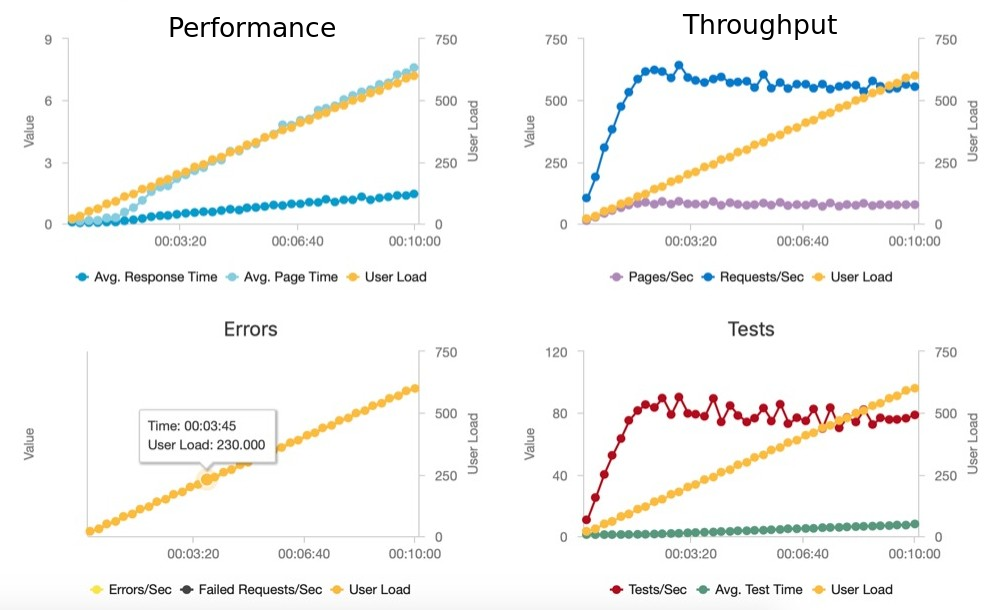
\includegraphics[width=170mm]{img/loadtest_01.png}
\caption{Results of a load test of the Kubernetes cluster. Most importantly from the \textit{Performance} chart it can be seen that Text Analytica's performance increases linearly when the number of users is increased. There is no significant loss in performance either.}
\label{img:loadtesting}
\end{figure*}

\section{Scalability}
\label{sec:scalability}
In a production environment, the number of Text Analytica users is expected to grow. As discussed in the lecture, sudden bursts in usage can sometimes not be foreseen \cite{Animoto}. Therefore, it was crucial to pay attention to the scalability of the application, to ensure a smooth and fast user experience independent of the number of parallel accesses. The application was built to handle an unknown number of users uploading and analysing files in parallel without running into errors or significant performance bottlenecks. In the remainder of this section it is discussed how this issue was addressed and results of one load test is shown.

\subsection{Infrastructure}
As mentioned in \Cref{sec:system-architecture} the web service is managed by a Kubernetes cluster. The main advantages of using a Kubernetes cluster are easy scalability and load balancing. More specifically, if usage of existing resources is high, the cluster will automatically scale \cite{KubernetesScaling, KubernetesAutoscaler}. In Text Analytica's case this might happen at peak times when a lot of people are using the Text Analytica web service. The cluster will then spawn more \textit{Pods} on the existing \textit{Azure VM Node}, to handle the additional workload without sacrificing performance \cite{MicrosoftAzureKubernetesService}.

When the \textit{Azure VM Node} is used to capacity new Pods are provisioned based on \textit{Virtual Kubelets} on a \textit{virtual node}. On the one hand this allows the application to start up new Pods faster, as there is no need to wait on new VMs being booted up as already explained in \Cref{subsec:infra}, on the other hand this enables “infinite” scaling as there is no capacity limit for a virtual node based on ACIs. Due to higher prices this option should, however, not be used permanently and in case of observing lasting high usage, more traditional VM-based nodes should be provisioned.

\subsection{Data storage}
Text Analytica uses an instance of Azure's \textit{Cosmos DB} for storage. The following part of this section discusses how scalability is addressed in terms of the data storage.

\textit{Cosmos DB} supports two kinds of partitioning: logical and physical partitions. Logical partition are such partitions, where all datasets or elements in a container share a property, which can serve as a partition key. In this case the data itself and the data throughput is automatically, horizontally partitioned and scaled by \textit{Cosmos DB}. Then there are the physical partitions. A number of logical partitions are assigned to one physical partition, which guarantees persistence and consistency of the data \cite{CosmosDBHorScal}. However, currently Text Analyticas database entries are not configured to have a partition key for logical partitioning. This is an improvement that eventually should be made.

\subsection{Monitoring and Load Testing}
To measure how well Text Analytica scales with an increasing workload respectively more parallel users we conducted a load test with the \textit{Azure DevOps} load testing solution \cite{AzureLoadTest}.

\Cref{img:loadtesting} displays the results of one of our load tests. The four diagrams show data for \textit{Performance}, \textit{Throughput}, \textit{Errors} and \textit{Tests}. The test lasted ten minutes and involved seven hundred virtual users at peak time, accessing the website. At this point we have not yet implemented a test case where actual files are uploaded to the application. From the \textit{Errors} diagram we observe that no errors occurred, which means our application did not fail even under high usage. The \textit{Performance} part contrasts the increasing user load, the increasing average response time as well as average page time. Interpreting this result, we conclude Text Analytica has a good scaling rate, as the response time scales nearly linear with no major increase in latency. The \textit{Throughput} figure shows the pages/sec and requests/sec with increasing user load, and \textit{Tests} simply shows the tests/sec and average test time.

A useful tool for monitoring the Kubernetes cluster is the \textit{Kubernetes Dashboard}. It shows all important resources, e.g. the number of Pods running, CPU and memory usage. This tool was especially helpful for debugging.

\section{Future improvements}
\label{sec:future-improvements}
As mentioned before, because of the time frame proposed for the development of this coursework project and especially due to initial issues with Oracle's cloud services, the submitted version of Text Analytica is just a prototype. Therefore there are some improvements on different levels, which are discussed in this section.

\subsection{Infrastructure}
At the moment, as Text Analytica has not much functionality, all of it is run on one container. To allow more specific scaling of certain parts of the application, the services should be split up into microservices, each running on its own container. Based on the current implementation the functionality could be split up into back-end, front-end and analysis. Not only would this separation allow for a more specific scaling of the services, but it would also allow to implement ingress rules, so that the ingress can be used as an application layer load balancer.

Another way to optimise Text Analytica would be improved management of the Kubernetes cluster itself. There are several popular open source projects, such as Istio, which can be used to efficiently manage a mesh of microservices \cite{Istio}.

A more drastic change to the system architecture would be the shift to serverless, implementing the different services as \textit{Azure functions} for example \cite{AzureFunctions}. Instead of the current IaaS approach, where some set up and maintenance has to be done by the user, this would mean using Azure's services on a PaaS level, allowing developers to focus on the application's functionality, while provisioning of resources and scaling is handled completely automatically by Azure.

\subsection{Service implementation}
As the focus of this coursework assignment was the application of cloud technologies and optimising the application for scaling, there are quite a few improvements on the service implementation level to be made in the future.

Firstly, there are some small bugs in the current implementation, such as the missing creation of an actual ID for the uploaded and analysed documents, which would need to be fixed. Secondly there is still some functionality missing to make Text Analytica an useful tool. Such functionality includes but is not limited to login and user account management, PDF uploads and processing, more advanced analysis as well as the option to store and retrieve files within or from the application.

To turn Text Analytica into a production level application it must comply to certain security standards. While developing the prototype there was no focus on security and therefore only minimal / default security measures are currently in place.

Lastly the existing continuous delivery pipeline could be extended for example by adding testing stages.

\section{Conclusion}
\label{sec:conclusion}
In this report, Text Analytica, a cloud-based web service for text analysis, was presented. The application is hosted on \textit{Microsoft Azure} and utilises a range of cloud computing technologies on IaaS and PaaS level.

The development of the project was described from the first conceptual vision to the implementation and testing of a fully functional prototype, based on Docker containers orchestrated by a Kubernetes cluster and an \textit{Azure Cosmos DB}. The discussion included elaborating on the platform choice, system architecture and scalability aspects. The results of a relatively simple load test, measuring the performance of the application under a high number of parallel site accesses, suggest Text Analytica is well suited for scaling.

Improvements to enhance the submitted prototype and eventually develop it into a production grade application, have been suggested.

\bibliographystyle{IEEEtran}
\bibliography{cw1-97059-97133}


\end{document}
